\documentclass{article}
\usepackage{tikz}
\usepackage{xcolor}
\usetikzlibrary{shapes,arrows}
\usetikzlibrary{calc}
\usepackage[dvipsnames]{xcolor}
\usepackage{listings}


\begin{document}

\begin{tikzpicture}
\tikzstyle{commit}=[draw,circle,fill=white,inner sep=0pt,minimum size=5pt]
\tikzstyle{every path}=[draw]
\tikzstyle{branch}=[draw,rectangle,rounded corners=3,fill=white,inner sep=2pt,minimum size=5pt]
% \node[commit, ForestGreen, fill=ForestGreen] (ef1eae1) at (0.0,0) {};
% \node[commit, Dandelion, fill=Dandelion] (4f669eb) at (0.5,-0.5) {};
% \node[right,xshift=10] (label_4f669eb) at (4f669eb.east) {\verb!4f669eb: Added README file with basic documentation!};
% \node[commit, Dandelion, fill=Dandelion] (9216cb2) at (0.5,-1.0) {};
% \node[right,xshift=10] (label_9216cb2) at (9216cb2.east) {\verb!9216cb2: Added a start message!};
% \node[commit, Red, fill=Red] (77c49c1) at (1.0,-1.5) {};
% \node[right,xshift=10] (label_77c49c1) at (77c49c1.east) {\verb!77c49c1: New script added.!};
% \node[commit, Dandelion, fill=Dandelion] (167af36) at (0.5,-2.0) {};
% \node[right,xshift=10] (label_167af36) at (167af36.east) {\verb!167af36: Added date/time to the final message in the script!};
% \path[Dandelion] (167af36) to[out=90,in=-90] (9216cb2);
% \path[Dandelion] (167af36) to[out=90,in=-90] (77c49c1);
% \node[commit, Dandelion, fill=Dandelion] (a2a2593) at (0.5,-2.5) {};
% \node[right,xshift=10] (label_a2a2593) at (a2a2593.east) {\verb!a2a2593: Merge branch 'Feature1'!};
% \path[Dandelion] (a2a2593) to[out=90,in=-90] (167af36);
% \node[commit, ForestGreen, fill=ForestGreen] (6ea97fa) at (0.0,-3.0) {};
% \node[right,xshift=10] (label_6ea97fa) at (6ea97fa.east) {\verb!6ea97fa: Added a line to the Feature1 branch!};
% \path[ForestGreen] (6ea97fa) to[out=90,in=-90] (ef1eae1);
% \path[ForestGreen] (6ea97fa) to[out=90,in=-90] (4f669eb);
% \path[ForestGreen] (6ea97fa) to[out=90,in=-90] (a2a2593);
% \node[commit, Dandelion, fill=Dandelion] (9f51c0d) at (0.5,-3.5) {};
% \node[right,xshift=10] (label_9f51c0d) at (9f51c0d.east) {\verb!9f51c0d: Added a 'finished' message at the end of the script!};
% \path[Dandelion] (9f51c0d) to[out=90,in=-90] (a2a2593);
% \node[commit, ForestGreen, fill=ForestGreen] (2e10426) at (0.0,-4.0) {};
% \node[right,xshift=10] (label_2e10426) at (2e10426.east) {\verb!2e10426: Added a line of text to my_file.txt.!};
% \path[ForestGreen] (2e10426) to[out=90,in=-90] (6ea97fa);
% \path[ForestGreen] (2e10426) to[out=90,in=-90] (9f51c0d);
% \node[commit, ForestGreen, fill=ForestGreen] (91f1fef) at (0.0,-4.5) {};
% \node[right,xshift=10] (label_91f1fef) at (91f1fef.east) {\verb!91f1fef: Converted another_file.txt to a Bash script.!};
% \path[ForestGreen] (91f1fef) to[out=90,in=-90] (2e10426);
% \node[commit, ForestGreen, fill=ForestGreen] (1ddccf6) at (0.0,-5.0) {};$
% \node[right,xshift=10] (label_1ddccf6) at (1ddccf6.east) {\verb!1ddccf6: Added a new file and added several lines to my_files.txt.!};
% \path[ForestGreen] (1ddccf6) to[out=90,in=-90] (91f1fef);
\node[commit, ForestGreen, fill=ForestGreen] (AAA) at (0.0,-5.5) {};
\node[right,xshift=10] (label_AAA) at (AAA.east) {\verb!AAA: This interdisciplinary course aims to give the student an understanding of performance and introduces foundations and state-of-the-art techniques in high performance software development.!};
% \path[ForestGreen] (AAA) to[out=90,in=-90] (1ddccf6);
\end{tikzpicture}

\end{document}